\documentclass[9pt]{extarticle}
% -- PACKAGES --
\usepackage[utf8]{inputenc} % UTF8 encoding
\usepackage[T1]{fontenc} % T1 font encoding (better for hyphenation, etc.)
\usepackage{lmodern} % Latin Modern font
\usepackage[margin=1in]{geometry} % Set margins
\usepackage{amsmath,amssymb,amsthm} % Math essentials
\usepackage{graphicx} % For including images
\usepackage[hidelinks]{hyperref} % Clickable hyperlinks in PDF
\usepackage{bookmark} % Helps manage bookmarks and outlines properly
\usepackage{cite} % Better citation handling
\usepackage[utf8]{inputenc} % Required for inputting international characters
\usepackage{graphicx}
\usepackage{algorithm}
\usepackage{algpseudocode}
\usepackage{mathtools}
\usepackage{bm}
\usepackage{tikz}
\usepackage{caption}
\usepackage{caption}
\usepackage{subcaption}
\usepackage{changepage}
\usetikzlibrary{decorations.pathreplacing, matrix, calc, positioning}

% -- THEOREM ENVIRONMENTS --
\theoremstyle{plain}
\newtheorem{theorem}{Theorem}[section]
\newtheorem{lemma}[theorem]{Lemma}

\theoremstyle{definition}
\newtheorem{definition}[theorem]{Definition}

\theoremstyle{remark}
\newtheorem{remark}[theorem]{Remark}



% -- TITLE & AUTHOR --
\title{Derivation and Implementation of a Multilayer Perceptron for MNIST Classification}
\author{Robert Davidson}
\date{\today}

\begin{document}


\begin{center}
    Mathematical Analysis of Multilayer Perceptron Training\\
    Independent / Self Study\\[24pt]
    \LARGE

    \Large
    \textbf{Robert Davidson}\\[6pt]
    \small
    BSc Mathematics and Computer Science \\ r.davidson1@universityofgalway.ie\\[6pt]
    Date: \today\\[12pt]
\end{center}
\begin{abstract}
    \begin{adjustwidth}{1cm}{1cm}
        This paper provides a comprehensive mathematical derivation and implementation of a Multilayer Perceptron (MLP)
        for the classification of handwritten digits from the MNIST dataset, starting from fundamental principles.
        We begin by exploring the biological inspiration behind artificial neurons, establishing a clear mapping between biological and artificial neural components.
        We then develop the mathematical representation of a single artificial neuron, progressing to the construction of perceptron layers and the full MLP architecture.
        The necessity of hidden layers for non-linear separability is discussed, alongside the selection and application of appropriate activation functions.
        We detail the forward propagation process using matrix-vector notation, followed by an in-depth explanation of cost functions and the error backpropagation algorithm
        for gradient computation. Optimization and training techniques, including batch-based methods and strategies for improving convergence, are examined.
        We address the critical issue of regularization to mitigate overfitting and underfitting, including the influence of initialization strategies.
        Finally, we present the implementation of a fully functional MLP for MNIST classification, concluding with a discussion of extensions to deeper architectures
        and modern practices in neural network development. This work aims to provide a clear, step-by-step mathematical foundation for understanding and building MLPs from the ground up.
    \end{adjustwidth}
\end{abstract}

\vspace{1.5cm}

\section*{Introduction}

The MNIST (Modified National Institute of Standards and Technology) dataset consists of
70,000 handwritten digit images (60,000 for training and 10,000 for testing).
It is commonly used for training and evaluating machine learning models in image recognition tasks.
Each image is a 28x28 pixel grayscale image, and the task is to classify the digit (0-9) represented by the image.



\begin{minipage}{0.3\textwidth}
    \centering
    
\includegraphics[scale = 0.15]{images/1_MNIST.png}
    \\ \textit{Sample MNIST digit 1}
\end{minipage}
\begin{minipage}{0.3\textwidth}
    \centering
    
\includegraphics[scale = 0.15]{images/2_MNIST.png}
    \\ \textit{Sample MNIST digit 2}
\end{minipage}
\begin{minipage}{0.3\textwidth}
    \centering
    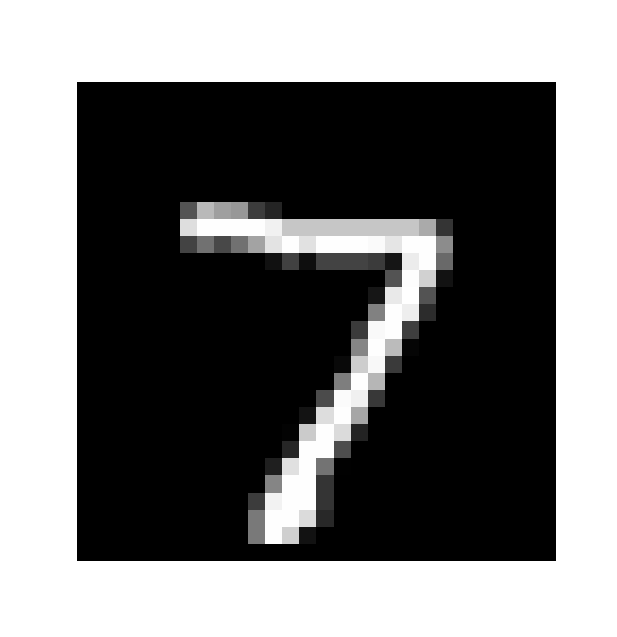
\includegraphics[scale = 0.15]{images/7_MNIST.png}
    \\ \textit{Sample MNIST digit 7}
\end{minipage}

\vspace{0.4cm}
\noindent A Multilayer Perceptron (MLP) is a type of artificial neural network composed of multiple
layers of nodes (neurons), each fully connected to the next layer. The MLP processes input data through
a series of transformations, with the final layer producing an output. It is one of the fundamental types
of neural networks and is used in a variety of applications, including image recognition. \\[2ex]
In this paper, we aim to build the mathematical foundations necessary to understand and implement a
Multilayer Perceptron (MLP) for the MNIST digit recognition task.

\pagebreak

\tableofcontents

\pagebreak
\section*{Preliminaries}
Here we will cover some basic mathematical concepts that will be used throughout the paper. These will be derived from first principles, so don't worry if you're not familiar with them.

\subsection*{Vectors}
A vector in mathematics is an ordered list of numbers, represented as a bold lowercase letter, e.g. $\mathbf{v}$. A vector can be represented as:
$$\mathbf{v} = \begin{bmatrix} v_1 \\ v_2 \\ \vdots \\ v_n \end{bmatrix}$$
We can refer to the first element as $v_1$, the second as $v_2$, and the $i$th element as $v_i$. \\
Each element of $\mathbf{v}$ corresponds to a coordinate in some $n$-dimensional space, where $n$ is just the number of elements in the vector. The vector points to the location of these coordinates in space. For example, take the vector in 2-dimensional space:
\begin{figure}[h]
    \begin{subfigure}[c]{0.48\textwidth}
        \centering
        $$\mathbf{v} = \begin{bmatrix} 2 \\ 1 \end{bmatrix}$$
    \end{subfigure}
    \begin{subfigure}[c]{0.48\textwidth}
        \centering
        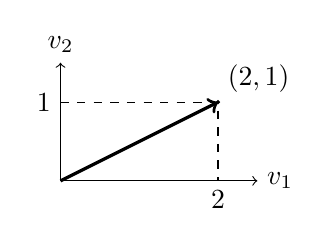
\begin{tikzpicture}
            \draw[->] (0,0) -- (2.5,0) node[right] {$v_1$};
            \draw[->] (0,0) -- (0,1.5) node[above] {$v_2$};
            \draw[->, very thick] (0,0) -- (2,1);
            \draw[dashed] (0,1) -- (2,1) -- (2,0);
            \node at (2,0) [below] {2};
            \node at (0,1) [left] {1};
            \filldraw (2,1) circle (0.5pt) node[above right] {$(2,1)$};
        \end{tikzpicture}
    \end{subfigure}
    \caption{A 2-dimensional vector $\mathbf{v}$}
\end{figure}

\subsection*{The Transpose of a Vector}
Consider a vector $\mathbf{v}$:
$$\mathbf{v} = \begin{bmatrix} v_1 \\ v_2 \\ \vdots \\ v_n \end{bmatrix}.$$
The transpose of $\mathbf{v}$, denoted $\mathbf{v}^T$, is the same vector, but flipped on its side:
$$\mathbf{v}^T = \begin{bmatrix} v_1 & v_2 & \ldots & v_n \end{bmatrix}.$$
The transpose of a vector is used to convert a row vector into a column vector, or vice versa.

\pagebreak

\subsection*{Multiplying Vectors : The Dot Product}
Say we have a vector $\mathbf{x} = \left[\begin{smallmatrix} x_1 \\ x_2 \end{smallmatrix}\right]$, we say the dimension of this is $2 \times 1$. In order to multiply $\mathbf{x}$ with another vector we need the vector to be of dimension $1 \times 2$. \\
Let $\mathbf{v} = \left[\begin{smallmatrix} v_1 \\ v_2 \end{smallmatrix}\right]$. We note that the dimension of $\mathbf{v}$ is $2 \times 1$. We can use the transpose of $v$ to turn it into a $1 \times 2$ vector.\\
Given two vectors $\mathbf{w}$ and $\mathbf{v}$:
$$\mathbf{w} = \begin{bmatrix} w_1 \\ w_2 \end{bmatrix} \quad \text{and} \quad \mathbf{v} = \begin{bmatrix} v_1 \\ v_2 \end{bmatrix}$$
\section{Motivation for the Multilayer Perceptron}
\begin{minipage}{0.7\textwidth}
    The perceptron is composed of multiple artificial neurons. Each of which makes a simple decision
    based on its inputs. These neurons are subsequently assembled into layers,
    with each layer functioning as a distinct 'area' of the brain.
    In this way, the Multilayer Perceptron serves as an abstract model inspired by the brain’s structure.
\end{minipage}
\begin{minipage}{0.29\textwidth}
    \centering
    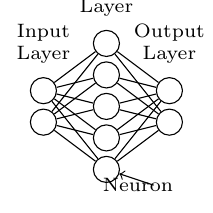
\begin{tikzpicture}[
            scale = 0.2, % reduced scale factor
            node distance=1.5cm,
            neuron/.style={circle, draw=black, minimum size=0.2cm},
            input/.style={neuron},
            hidden/.style={neuron},
            output/.style={neuron},
            layer/.style={text width=2cm, text centered, font=\scriptsize}
        ]

        \useasboundingbox (-1, -4) rectangle (9, 6);
        \node[layer] (input-label) at (0,5) {Input \\ Layer};
        \node[layer] (hidden-label) at (4,8) {Hidden \\ Layer};
        \node[layer] (output-label) at (8,5) {Output \\ Layer};



        % Input layer nodes
        \node[input] (I-1) at (0,2) {};
        \node[input] (I-2) at (0,0) {};


        % Hidden layer nodes
        \node[hidden] (H-1) at (4,5) {};
        \node[hidden] (H-2) at (4,3) {};
        \node[hidden] (H-3) at (4,1) {};
        \node[hidden] (H-4) at (4,-1) {};
        \node[hidden] (H-5) at (4,-3) {};


        % Output layer nodes
        \node[output] (O-1) at (8,2) {};
        \node[output] (O-2) at (8,0) {};

        % Connections between input and hidden layer
        \foreach \i in {1,2}
        \foreach \j in {1,2,3,4,5}
        \draw[-] (I-\i) -- (H-\j);

        % Connections between hidden and output layer
        \foreach \i in {1,2,3,4,5}
        \foreach \j in {1,2}
        \draw[-] (H-\i) -- (O-\j);

        \draw[->] (7,-4) -- (H-5);
        \node at (6,-4) {\scriptsize Neuron};

    \end{tikzpicture}
\end{minipage}


\subsection{The Structure and Function of a Biological Neuron}
Neurons, the brain’s fundamental processing units, transmit information
throughout the nervous system. The human brain contains about 86 billion
neurons \cite{harvard_brain}, each comprising:
\begin{itemize}
    \item \textbf{Dendrites:} Branch-like structures that receive input signals from other neurons.
    \item \textbf{Cell Body (Soma):} Combines incoming signals and determines whether the neuron should fire.
    \item \textbf{Axon:} Carries the electrical impulse (if the combined signal at the soma exceeds the threshold) to other neurons.
    \item \textbf{Synapse:} Junction between neurons; connects one neuron's axon to another's dendrites.
    \item \textbf{Firing Threshold} The neuron fires only if the total input exceeds a certain threshold.
\end{itemize}
\subsection{Mapping the Biological Neuron to the Artificial Neuron}
The perceptron, proposed by Frank Rosenblatt in 1958 \cite{rosenblatt_perceptron}, is a simplified model of the biological neuron. Its components are:
\begin{itemize}
    \item \textbf{Inputs:} $x_1, x_2, \ldots, x_n$, analogous to dendrites.
    \item \textbf{Weights:} $w_1, w_2, \ldots, w_n$, indicating each input's importance.
    \item \textbf{Summation:} $\sum w_i x_i + b$, analogous to the soma, with $b$ as a bias term.
    \item \textbf{Activation Function $(\boldsymbol{\phi})$:} applies a mathematical function to the weighted sum to determine the output $y$, analogous to the neuron's firing mechanism.
    \item \textbf{Output:} The final signal from the perceptron.
\end{itemize}

\begin{figure}[h]
    \centering
    \begin{subfigure}[b]{0.48\textwidth}
        \centering
        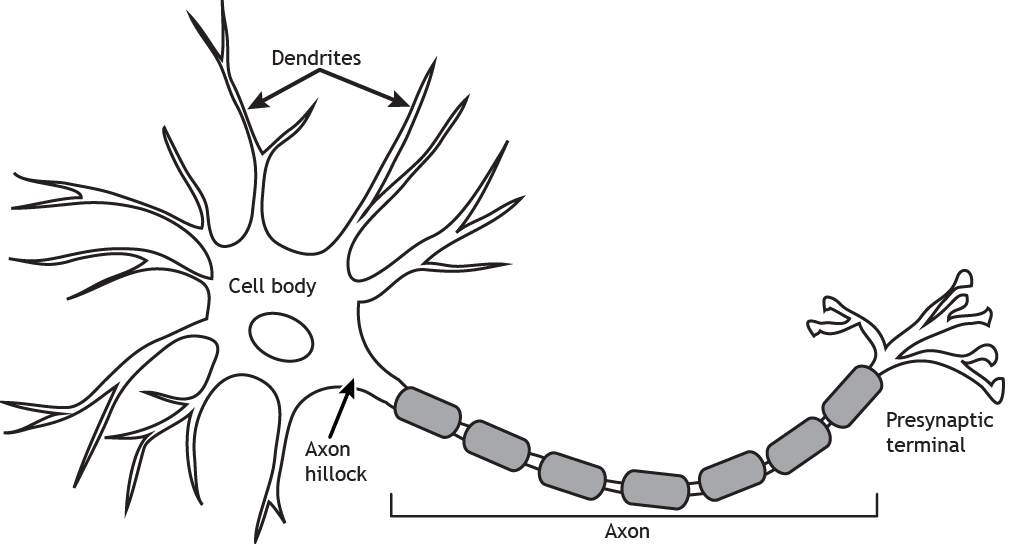
\includegraphics[scale=0.2]{images/humanNeuron.png}
        \caption{Human neuron \cite{human_neuron}}
    \end{subfigure}
    \hfill
    \begin{subfigure}[b]{0.48\textwidth}
        \centering
        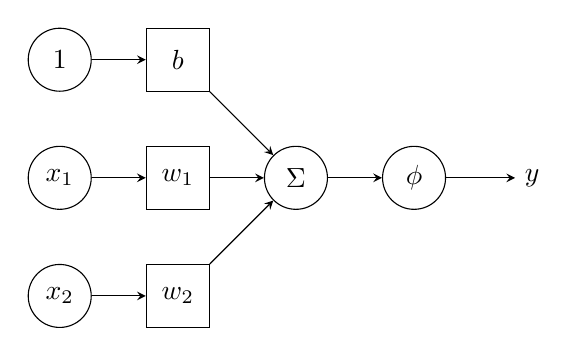
\begin{tikzpicture}[>=stealth, node distance=2.5cm, auto]

            % Draw the two input variables and the bias term
            \node[draw, circle, minimum size=0.8cm] (x0) at (0,1.5) {$1$};
            \node[draw, circle, minimum size=0.8cm] (x1) at (0,0) {$x_1$};
            \node[draw, circle, minimum size=0.8cm] (x2) at (0,-1.5) {$x_2$};


            % Draw the weights 
            \node[draw, rectangle, minimum size =0.8cm] (w0) at (1.5,1.5) {$b$};
            \node[draw, rectangle, minimum size =0.8cm] (w1) at (1.5,0) {$w_1$};
            \node[draw, rectangle, minimum size =0.8cm] (w2) at (1.5,-1.5) {$w_2$};

            % Draw the summation 
            \node[draw, circle, minimum size=0.8cm] (p) at (3,0) {$\Sigma$};

            \node[draw, circle, minimum size=0.8cm] (a) at (4.5,0) {$\phi$};

            % Draw the output 
            \node at (6,0) (y) {$y$};

            % Arrows connecting inputs to weights
            \draw[->] (x0) -- (w0);
            \draw[->] (x1) -- (w1);
            \draw[->] (x2) -- (w2);

            % Arrows connecting weights to summation
            \draw[->] (w0) -- (p);
            \draw[->] (w1) -- (p);
            \draw[->] (w2) -- (p);

            % Arrow connecting summation to activation function
            \draw[->] (p) -- (a);

            % Arrow connecting activation function to output
            \draw[->] (a) -- (y);


        \end{tikzpicture}
        \caption{Artificial neuron}
    \end{subfigure}
    \caption{Comparison of biological and artificial neurons.}
\end{figure}


\pagebreak

\section{Artificial Neurons}

\subsection{Mathematical Representation}
To represent the artificial neueron, we'll start with an example, two inputs $x_1$ and $x_2$ into a neueron $h_1$.
\begin{figure}[h]
    \centering
    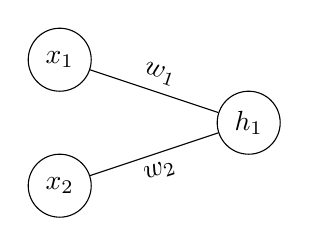
\begin{tikzpicture}[>=stealth, node distance=2.5cm, auto, scale=0.8]

        % Draw the two input variables and the bias term

        \node[draw, circle, minimum size=0.8cm] (x1) at (0,1) {$x_1$};
        \node[draw, circle, minimum size=0.8cm] (x2) at (0,-1) {$x_2$};

        % Draw the summation 
        \node[draw, circle, minimum size=0.8cm] (p) at (3,0) {$h_1$};

        % Arrows connecting inputs to weights

        \draw[-] (x1) -- (p) node[midway, sloped, above] {$w_1$};
        \draw[-] (x2) -- (p) node[midway, sloped, below] {$w_2$};
    \end{tikzpicture}
\end{figure} \\
\textbf{Finding the total input} $\mathbf{(z)}$\\[2ex]
We could do this by adding up each input multiplied by its weight - indicating how important it is..
$$z = w_1 \cdot x_1 + w_2 \cdot x_2$$
To make this easier for us, we could represent the weights and inputs as vectors:
$$\mathbf{w} = \begin{bmatrix} w_1 \\ w_2 \end{bmatrix} \quad \text{and} \quad \mathbf{x} = \begin{bmatrix} x_1 \\ x_2 \end{bmatrix}$$
We then see then see that we can write:
$$z = [w_1, w_2] \cdot \begin{bmatrix} x_1 \\ x_2 \end{bmatrix} = w_1 \cdot x_1 + w_2 \cdot x_2$$
We can see that $[w_1, w_2]$ is just out weights vector transposed. We can write this as:
$$z = \mathbf{w}^T \mathbf{x}$$
\textbf{Applying the Activation Function} $\boldsymbol{(\phi)}$\\[2ex]
We introduce the Heaviside step activation function – which is like an on-off switch. If the total input is greater than $0$, the neuron fires; otherwise it doesn't.
\begin{figure}[h]
    \centering
    \begin{subfigure}[c]{0.49\textwidth}
        \centering
        $$\phi(z) = \begin{cases}
                1 & \text{if } z \geq 0 \\
                0 & \text{if } z < 0
            \end{cases}
        $$
    \end{subfigure}
    \begin{subfigure}[c]{0.5\textwidth}
        \centering
        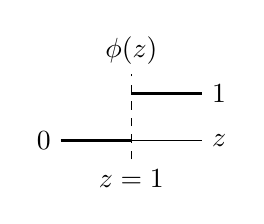
\begin{tikzpicture}[scale = 0.6]
            \draw[-] (-1.5,0) -- (1.5,0) node[right] {$z$};
            \draw[very thick] (-1.5,0) -- (0,0);
            \draw[very thick] (0,1) -- (1.5,1);
            \draw[dashed] (0,-0.4) -- (0,1.4);
            \node at (1.5,1) [right] {1};
            \node at (-1.5,0) [left] {0};
            \node at (0,-0.4) [below] {$z = 1$};
            \node at (0,1.4) [above] {$\phi(z)$};
        \end{tikzpicture}
    \end{subfigure}
    \caption{The Heaviside step function}
\end{figure} \\
\textbf{Introducing the bias} $\boldsymbol{(b)}$\\[2ex]
What is we want to change how much of a total input it takes for a neuron to fire? We can introduce a bias term $b$ to the total input:
$$z = \mathbf{w}^T \mathbf{x} + b$$
This allows us to shift the total input by an amount $b$. Which makes the activation function look like:
\begin{figure}[h]
    \centering
    \begin{subfigure}[t]{0.49\textwidth}
        \centering
        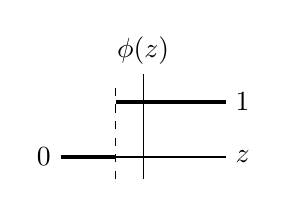
\begin{tikzpicture}[scale = 0.7]
            \draw[-] (0,-0.4) -- (0,1.5) node[above] {$\phi(z)$};
            \draw[-] (-1.5,0) -- (1.5,0) node[right] {$z$};
            \draw[very thick] (-1.5,0) -- (-0.5,0);
            \draw[very thick] (-0.5,1) -- (1.5,1);
            \draw[dashed] (-0.5,-0.4) -- (-0.5,1.4);
            \node at (1.5,1) [right] {1};
            \node at (-1.5,0) [left] {0};
        \end{tikzpicture}
        \caption{$b = 0.5$}
    \end{subfigure}
    \begin{subfigure}[t]{0.49\textwidth}
        \centering
        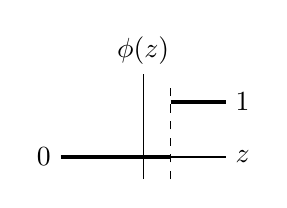
\begin{tikzpicture}[scale = 0.7]
            \draw[-] (0,-0.4) -- (0,1.5) node[above] {$\phi(z)$};
            \draw[-] (-1.5,0) -- (1.5,0) node[right] {$z$};
            \draw[very thick] (-1.5,0) -- (0.5,0);
            \draw[very thick] (0.5,1) -- (1.5,1);
            \draw[dashed] (0.5,-0.4) -- (0.5,1.4);
            \node at (1.5,1) [right] {1};
            \node at (-1.5,0) [left] {0};
        \end{tikzpicture}
        \caption{$b = -0.5$}
    \end{subfigure}
    \caption{The effect of the bias term on the activation function}
\end{figure}

\pagebreak

\subsection{Learning}
The core idea of learning is, given an unfavorable outcome, we look back and try to figure out what we could've done
differently to achieve a better outcome.
We can only do this if we know how wrong our decision was, and what we should have done instead. \\[2ex]
Consider, for a moment , getting a college test result back. If we wanted to get 90\% on the test and only got 40\%, we know
we need to give a much higher weight to studying next time. Whereas, if we got 88\% we know we're on the right track, and
only need to make minor adjustments. \\[2ex]
In an artificial neuron, we can compare the difference between the correct output and the output produced by the neuron.
The larger the error, the greater need for adjustment.
The learning rate $\eta$ controls how sensitive we are to these errors. A high learning rate means we make large adjustments,
while a low learning rate means we make small adjustments. \\[2ex]
The question then becomes, why not always use a high learning
rate? Let's revisit the college test scenario. Imagine you
aimed for 90\% but only scored 40\%. A large error signal indicates a
significant adjustment is needed. With a high learning rate,
you would react very strongly to this error. You might drastically
increase your study time, perhaps even overcompensating and studying excessively.
This could lead to burnout or neglecting other important aspects of life.
Conversely, with a low learning rate, even with a 40\% score, your adjustment would be small.
You might only slightly increase your study time, potentially not enough to significantly improve your score on the next test. The learning rate, therefore, is a delicate balance. It needs to be high enough to enable learning in a reasonable time, but low enough to prevent wild oscillations or overreactions to errors.
The learning rate, is something we can adjust to find the right balance between making large adjustments when we are far off,
and making small adjustments when we are close to the correct answer. \\[2ex]
Mathematically, we can represent the learning process as follows.
We define the error as the difference between the predicted result and the actual result.
This error indicates how far off our prediction was from the correct answer, and can be positive (overprediction) or negative (underprediction)
$$\text{Error} = y_{\text{actual}} - y_{\text{predicted}}$$
We then define how much we should change the weight of each input $(x_i)$ as:
$$\Delta w_i = \eta \times \text{Error} \times x_i$$
Here, $\eta$ is the learning rate, controlling our sensitivity to errors.
The multiplication by $x_i$is important because it scales the weight adjustment by the magnitude of the input $x_i$.
Inputs with larger values have a proportionally larger influence on the output,
and therefore their weights should be adjusted more significantly for a given error.
We also calculate the change for the bias term as:
We also calculate how much we should change the bias term as:
$$\Delta b = \eta \times \text{Error}$$
The intuition behind these adjustments is that if the prediction is consistently too low, we increase weights and bias to make firing easier (like studying more).
If consistently too high, we decrease them to make firing harder (like studying less). We then update the weights and bias as follows:
$$w_i = w_i + \Delta w_i$$
$$b = b + \Delta b$$


\pagebreak

\subsection{What does the Artificial Neuron Actually do? - Example: Mushroom Classification}
Imagine we're in a field filled with all kinds of mushrooms. Some have dozens of little white spots, and tall stems. While others have very few spots and short terms.
You know from past experience that the mushrooms with many spots are poisonous, while the ones with few spots are safe to eat. \\[2ex]
But there's a catch. Sometimes we find mushrooms that are hard to classify - they have medium length stems, or only a few spots. Where exactly do we draw the line between poisonous and safe mushrooms? You may not know from a glance, and you
certainly don't want to eat a poisonous mushroom to find out. \\[2ex]
This is exactly the problem the artificial neuron helps solve. It learns to draw a line in the mushroom field that separates the poisonous mushrooms from the safe ones.\\
Lets define the two inputs to our neueron as:
$$x_1 = \text{number of spots} \quad \text{and} \quad x_2 = \text{length of the stem}$$
The artificial neueron then forms a linear combination of these inputs:
$$z = \sum_{i=1}^{2} w_i x_i + b = w_1 x_1 + w_2 x_2 + b \Rightarrow z = \mathbf{w}^T \mathbf{x} + \mathbb{b}$$

where our weights scale the importance of each input.
The neueron then decides whether the mushroom is poisonous or not:
$$
    y = \begin{cases}
        1 & \text{if } z \geq 0 \\
        0 & \text{if } z < 0
    \end{cases}
$$
where, $y = 1$ means the mushroom is poisonous, and $y = 0$ means it is safe to eat. The perceptron learns the weights $w_1$ and $w_2$ to draw the best line that separates the two classes of mushrooms.

\begin{figure}[h]
    \centering
    \begin{subfigure}{0.3\textwidth}
        \centering
        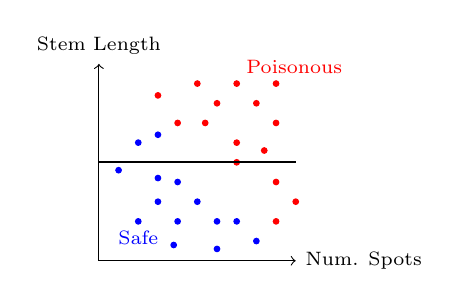
\begin{tikzpicture}[scale=0.5]
            % axes
            \draw[->] (0,0) -- (5,0) node[right] {\scriptsize Num. Spots};
            \draw[->] (0,0) -- (0,5) node[above] {\scriptsize Stem Length};

            % sample points: safe (blue) and poisonous (red)
            \filldraw[blue] (1,1) circle (2pt) node[below] {\scriptsize Safe};
            \filldraw[blue] (2,2) circle (2pt);
            \filldraw[blue] (2.5,1.5) circle (2pt);
            \filldraw[blue] (3,1) circle (2pt);
            \filldraw[blue] (0.5,2.3) circle (2pt);
            \filldraw[blue] (1.5,1.5) circle (2pt);
            \filldraw[blue] (3.5,1) circle (2pt);
            \filldraw[blue] (3,0.3) circle (2pt);
            \filldraw[blue] (4,0.5) circle (2pt);
            \filldraw[blue] (2,1) circle (2pt);
            \filldraw[blue] (1.9,0.4) circle (2pt);
            \filldraw[blue] (1.5,2.1) circle (2pt);
            \filldraw[blue] (1,3) circle (2pt);
            \filldraw[blue] (1.5,3.2) circle (2pt);


            \filldraw[red] (3.5,3) circle (2pt) ;
            \filldraw[red] (4,4) circle (2pt);
            \filldraw[red] (3,4) circle (2pt);
            \filldraw[red] (4.5,3.5) circle (2pt);
            \filldraw[red] (4.2,2.8) circle (2pt);
            \filldraw[red] (3.5,2.5) circle (2pt);
            \filldraw[red] (2,3.5) circle (2pt);
            \filldraw[red] (2.7,3.5) circle (2pt);
            \filldraw[red] (4.5,1) circle (2pt);
            \filldraw[red] (4.5,2) circle (2pt);
            \filldraw[red] (1.5,4.2) circle (2pt);
            \filldraw[red] (5,1.5) circle (2pt);
            \filldraw[red] (2.5,4.5) circle (2pt);
            \filldraw[red] (3.5,4.5) circle (2pt) node[above right] {\scriptsize Poisonous};
            \filldraw[red] (4.5,4.5) circle (2pt);

            \draw[thick] (0,2.5) -- (5,2.5);
        \end{tikzpicture}
        \caption{Before training}
    \end{subfigure}
    \begin{subfigure}{0.3\textwidth}
        \centering
        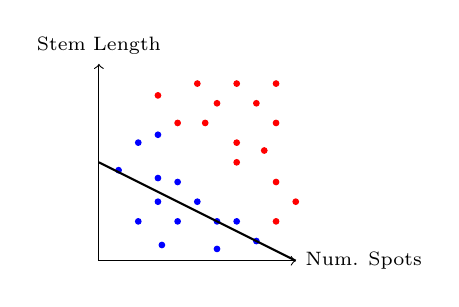
\begin{tikzpicture}[scale=0.5]
            % axes
            \draw[->] (0,0) -- (5,0) node[right] {\scriptsize Num. Spots};
            \draw[->] (0,0) -- (0,5) node[above] {\scriptsize Stem Length};

            % sample points: safe (blue) and poisonous (red)
            \filldraw[blue] (1,1) circle (2pt);
            \filldraw[blue] (2,2) circle (2pt);
            \filldraw[blue] (2.5,1.5) circle (2pt);
            \filldraw[blue] (3,1) circle (2pt);
            \filldraw[blue] (0.5,2.3) circle (2pt);
            \filldraw[blue] (1.5,1.5) circle (2pt);
            \filldraw[blue] (3.5,1) circle (2pt);
            \filldraw[blue] (3,0.3) circle (2pt);
            \filldraw[blue] (4,0.5) circle (2pt);
            \filldraw[blue] (2,1) circle (2pt);
            \filldraw[blue] (1.6,0.4) circle (2pt);
            \filldraw[blue] (1.5,2.1) circle (2pt);
            \filldraw[blue] (1,3) circle (2pt);
            \filldraw[blue] (1.5,3.2) circle (2pt);


            \filldraw[red] (3.5,3) circle (2pt);
            \filldraw[red] (4,4) circle (2pt);
            \filldraw[red] (3,4) circle (2pt);
            \filldraw[red] (4.5,3.5) circle (2pt);
            \filldraw[red] (4.2,2.8) circle (2pt);
            \filldraw[red] (3.5,2.5) circle (2pt);
            \filldraw[red] (2,3.5) circle (2pt);
            \filldraw[red] (2.7,3.5) circle (2pt);
            \filldraw[red] (4.5,1) circle (2pt);
            \filldraw[red] (4.5,2) circle (2pt);
            \filldraw[red] (1.5,4.2) circle (2pt);
            \filldraw[red] (5,1.5) circle (2pt);
            \filldraw[red] (2.5,4.5) circle (2pt);
            \filldraw[red] (3.5,4.5) circle (2pt);
            \filldraw[red] (4.5,4.5) circle (2pt);

            \draw[thick] (0,2.5) -- (5,0);
        \end{tikzpicture}
        \caption{After 100 training passes (epochs)}
    \end{subfigure}
    \begin{subfigure}{0.3\textwidth}
        \centering
        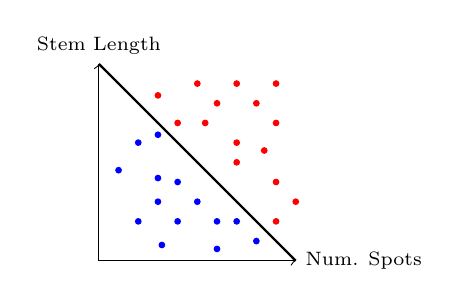
\begin{tikzpicture}[scale=0.5]
            % axes
            \draw[->] (0,0) -- (5,0) node[right] {\scriptsize Num. Spots};
            \draw[->] (0,0) -- (0,5) node[above] {\scriptsize Stem Length};

            % sample points: safe (blue) and poisonous (red)
            \filldraw[blue] (1,1) circle (2pt);
            \filldraw[blue] (2,2) circle (2pt);
            \filldraw[blue] (2.5,1.5) circle (2pt);
            \filldraw[blue] (3,1) circle (2pt);
            \filldraw[blue] (0.5,2.3) circle (2pt);
            \filldraw[blue] (1.5,1.5) circle (2pt);
            \filldraw[blue] (3.5,1) circle (2pt);
            \filldraw[blue] (3,0.3) circle (2pt);
            \filldraw[blue] (4,0.5) circle (2pt);
            \filldraw[blue] (2,1) circle (2pt);
            \filldraw[blue] (1.6,0.4) circle (2pt);
            \filldraw[blue] (1.5,2.1) circle (2pt);
            \filldraw[blue] (1,3) circle (2pt);
            \filldraw[blue] (1.5,3.2) circle (2pt);


            \filldraw[red] (3.5,3) circle (2pt);
            \filldraw[red] (4,4) circle (2pt);
            \filldraw[red] (3,4) circle (2pt);
            \filldraw[red] (4.5,3.5) circle (2pt);
            \filldraw[red] (4.2,2.8) circle (2pt);
            \filldraw[red] (3.5,2.5) circle (2pt);
            \filldraw[red] (2,3.5) circle (2pt);
            \filldraw[red] (2.7,3.5) circle (2pt);
            \filldraw[red] (4.5,1) circle (2pt);
            \filldraw[red] (4.5,2) circle (2pt);
            \filldraw[red] (1.5,4.2) circle (2pt);
            \filldraw[red] (5,1.5) circle (2pt);
            \filldraw[red] (2.5,4.5) circle (2pt);
            \filldraw[red] (3.5,4.5) circle (2pt);
            \filldraw[red] (4.5,4.5) circle (2pt);

            \draw[thick] (0,5) -- (5,0);
        \end{tikzpicture}
        \caption{Final decision boundary}
    \end{subfigure}
    \caption{Artificial Neuron learning to separate safe and poisonous mushrooms.}
\end{figure}
We refer to this line as the decision boundary, as it separates the two classes of mushrooms. We now have a simple model, that given the number of spots and the length of the stem, can predict whether a mushroom is poisonous or safe to eat. This is the essence of what an artificial neuron does - it learns to draw decision boundaries in the input space to separate different classes of data.

In essence, an artificial neuron integrates multiple inputs by scaling them with weights, adds a bias to adjust the activation threshold, and passes the resulting sum through a non-linear activation function. Its learning process—driven by error correction—enables it to modify its parameters to better approximate the desired output. This rigorous yet intuitive framework is the cornerstone of more complex neural network architectures.

\pagebreak


\section{A Layer of Neurons}
\subsection{Recap of the Single Neuron and Intro to Layers}
The artificial neuron is a simple unit, like a tiny decision maker. It takes inputs representing different features (think stems and spots of mushrooms), it gives these features different weights (importance), adds them up, applies a little tweak (a bias) and runs it through an activation function (like a yes/no switch) to decide what to output. It learns by tweaking these weights and biases to make better decisions on examples its given. \\ [2ex]
Now, instead of one neuron working alone, we introduce a layer of neurons, each of them looking at the same inputs but looking at them in different ways, for example one might focus on the color of the mushroom, while another might focus on its size. Together, these neurons can work together to make more complex decisions, where we can consider multiple features at once.

\subsection{The XOR Problem}
A single artificial neuron can separate data with only one straight line—great if your data is linearly separable. But some datasets require more complex boundaries. One classic example is the XOR (exclusive OR) problem: how do we classify data points that should be labeled “1” if they satisfy exactly one condition (but not both), and “0” otherwise?

\vspace{1em} \noindent \textbf{Analogy: A Chef and Two Flavors}

\noindent Imagine a chef wants to create a dish that is appealing only if it is \textit{either} sweet \textit{or} spicy, but not both (that combination clashes) and not neither (too boring). This is precisely the XOR condition: the dish is appealing if it is sweet \textit{or} spicy, but not both. The chef needs to find the right balance of flavors to create a dish that satisfies this condition.

\begin{figure}[h]
    \centering
    \begin{subfigure}[b]{0.45\textwidth}
        \centering
        \begin{tabular}{|c|c|c|}
            \hline
            \textbf{Sweet} & \textbf{Spicy} & \textbf{Dish}              \\
            \hline
            \text{No}      & \text{No}      & \text{No \;(boring dish)}  \\
            \hline
            \text{No}      & \text{Yes}     & \text{Yes (sweet dish)}    \\
            \hline
            \text{Yes}     & \text{No}      & \text{Yes (spicy dish)}    \\
            \hline
            \text{Yes}     & \text{Yes}     & \text{No (flavours clash)} \\
            \hline
        \end{tabular}
        \caption{XOR truth table}
    \end{subfigure}
    \hfill
    \begin{subfigure}[b]{0.45\textwidth}
        \centering
        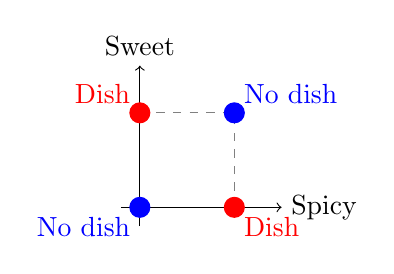
\begin{tikzpicture}[scale=1.2]
            % grid lines for clarity
            \draw[dashed, gray] (0,1) -- (1,1);
            \draw[dashed, gray] (1,0) -- (1,1);
            % axes
            \draw[->] (-0.2,0) -- (1.5,0) node[right] {$\text{Spicy}$};
            \draw[->] (0,-0.2) -- (0,1.5) node[above] {$\text{Sweet}$};

            % points
            \filldraw[blue] (0,0) circle (3pt) node[below left] {\text{No dish}};
            \filldraw[red] (0,1) circle (3pt) node[above left] {\text{Dish}};
            \filldraw[red] (1,0) circle (3pt) node[below right] {\text{Dish}};
            \filldraw[blue] (1,1) circle (3pt) node[above right] {\text{No dish}};
        \end{tikzpicture}
        \caption{Visualization of XOR: Red = 1, Blue = 0}
    \end{subfigure}
    \caption{The XOR problem}
\end{figure}
As we can see, we can't split this data with a single straight line so that all the red points are one side and all the blue points are on the other side. This is where a single neuron fails. We need a more complex decision boundary. To solve this problem we can use multiple neurons in the same layer, where each neueron draws its own boundry ad the final decision is made by combining the outputs of these neurons. \\[2ex]
Returning to the chef analogy: the chef might hire two sous-chefs. One sous-chef checks sweetness ($N_1$); the other checks spiciness ($N_2$). Their “votes” are then combined in a final decision. In neural network terms, each neuron in the hidden layer focuses on a specific aspect of the input; then the outputs are aggregated by the next neuron. This layering of simpler decisions leads to richer, non-linear decision boundaries—enabling the network to classify the XOR data correctly.

\begin{figure}[h]
    \begin{subfigure}[b]{0.45\textwidth}
        \begin{center}
            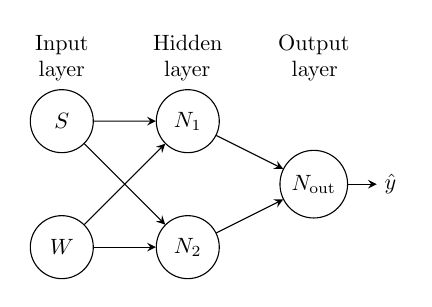
\begin{tikzpicture}[>=stealth, node distance=2cm, scale=0.8, transform shape]
                \node[align=left] at (0,2) {Input \\ \,layer};
                \node[draw, circle, minimum size=1cm] (S) at (0,1) {$S$};
                \node[draw, circle, minimum size=1cm] (W) at (0,-1) {$W$};

                \node[align=left] at (2,2) {Hidden \\ \, layer};
                \node[draw, circle, minimum size=1cm] (N1) at (2,1) {$N_1$};
                \node[draw, circle, minimum size=1cm] (N2) at (2,-1) {$N_2$};

                \node[align=left] at (4,2) {Output \\ \; layer};
                \node[draw, circle, minimum size=1cm] (Nout) at (4,0) {$N_{\mathrm{out}}$};

                % Connections: inputs to hidden
                \draw[->] (S) -- (N1);
                \draw[->] (S) -- (N2);
                \draw[->] (W) -- (N1);
                \draw[->] (W) -- (N2);

                % Connections: hidden to output
                \draw[->] (N1) -- (Nout);
                \draw[->] (N2) -- (Nout);

                % Label the final output
                \node[right] at (5,0) {$\hat{y}$};
                \draw[->] (Nout) -- (5,0);
            \end{tikzpicture}
        \end{center}
        \subcaption{Architecture of the chef analogy}
    \end{subfigure}
    \hfill
    \begin{subfigure}[b]{0.5\textwidth}
        \centering
        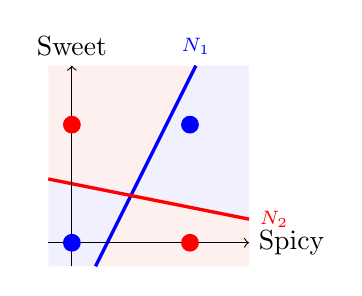
\begin{tikzpicture}[scale=1.5]
            % Define clipping rectangle (limits of our drawing)
            \begin{scope}
                \clip (-0.2,-0.2) rectangle (1.5,1.5);

                \fill[blue!20, opacity=0.3]
                (0.5,0.45) -- (1.5,0.2) -- (1.5,1.5) -- (1.05,1.5) -- cycle;

                \fill[blue!20, opacity=0.3]
                (0.5,0.45) -- (-0.2,0.54) -- (-0.2,-0.2) -- (0.2,-0.2) -- cycle;


                \fill[red!20, opacity=0.3]
                (0.5,0.45) -- (-0.2,0.54) -- (-0.2,1.5) -- (1.05,1.5) -- cycle;

                \fill[red!20, opacity=0.3]
                (0.5,0.45) -- (1.5,0.2) -- (1.5,-0.2) -- (0.2,-0.2) -- cycle;
            \end{scope}

            % Draw decision boundaries
            \draw[very thick, blue] (0.2,-0.2) -- (1.05,1.5) node[above] {\scriptsize$N_1$};
            \draw[very thick, red] (-0.2,0.54) -- (1.5,0.2) node[right] {\scriptsize$N_2$};

            % Draw axes
            \draw[->] (-0.2,0) -- (1.5,0) node[right, black] {Spicy};
            \draw[->] (0,-0.2) -- (0,1.5) node[above, black] {Sweet};

            % Draw points
            \filldraw[blue] (0,0) circle (2pt) node[below left] {};
            \filldraw[red] (0,1) circle (2pt) node[above left] {};
            \filldraw[red] (1,0) circle (2pt) node[below right] {};
            \filldraw[blue] (1,1) circle (2pt) node[above right] {};
        \end{tikzpicture}
        \subcaption{Decision boundaries}
    \end{subfigure}
    \caption{A layer of neurons for the XOR problem}
\end{figure}

\section{Why stop at one layer?}
The XOR problem (chef anology) is a small illustration on non-linearly seperable problems. Most real word tasks have layers of complextity that drawf the XOR example. For example:
\begin{itemize}
    \item \textbf{Image Recognition}: Deciding whethera cat or dog involves thousdands or millions of pixels. A single layer of neueron cannot capture the patterns of edges, shapes, and textures that define a cat or dog.
    \item \textbf{Natural Language Processing}: Understanding a sentence involves understanding the meaning of each word, the context in which they are used, and the relationships between them. A single layer of neurons cannot capture the complexity of language.
\end{itemize}
\subsection{The Power of Chaining Layers}
Just having one layer of neurons is like having a single sous-chef in the kitchen. They can only focus on one aspect of the dish. To create a complex dish, the chef needs multiple sous-chefs, each focusing on different aspects of the dish. Similarly, to solve complex problems, we need multiple layers of neurons, each layer focusing on different aspects of the input data. This is the essence of deep learning: using multiple layers of neurons to learn complex patterns in data.\\[2ex]
One way to overcome these limitations is to chain mutliple layers of neuerons so that the output of one layer becomes the input of the next. For example, in image recoginition, one layer might learn to respond to simple edges or colors, while the next layer might take these edges as inputs and learn to detect more complex shapes, like corners and textures, a third layer might combine these shapes into an understanding of objects like a cats ear, or a dogs nose. This chaining of layers is what gives deep learning its name.
\begin{figure}[h]
    \begin{center}
        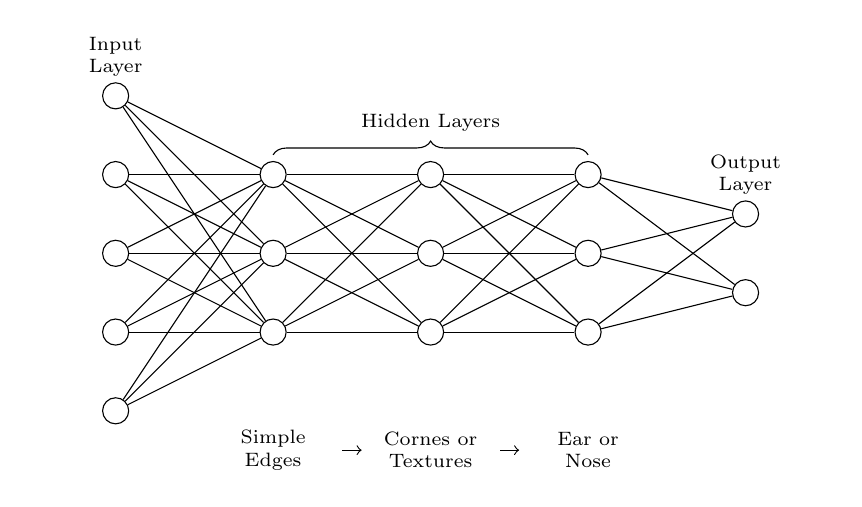
\begin{tikzpicture}[
                scale = 1,
                node distance=1.5cm,
                neuron/.style={circle, draw=black, minimum size=0.2cm},
                input/.style={neuron},
                hidden/.style={neuron},
                output/.style={neuron},
                layer/.style={text width=2cm, text centered, font=\scriptsize}
            ]


            \node[layer] (input-label) at (0,2.5) {Input \\ Layer};
            \draw [decorate,decoration={brace,amplitude=5pt}]
            (2,1.25) -- (6,1.25) node[midway, above, yshift=0.5em]{\scriptsize Hidden Layers};
            \node[layer] (output-label) at (8,1) {Output \\ Layer};

            \node[layer] (hidden-label-1) at (2,-2.5) {Simple \\ Edges};
            \node[layer] (hidden-label-2) at (4,-2.5) {Cornes or \\Textures};
            \node[layer] (hidden-label-3) at (6,-2.5) {Ear  or\\ Nose};



            % Input layer nodes
            \node[input] (I-1) at (0,2) {};
            \node[input] (I-2) at (0,1) {};
            \node[input] (I-3) at (0,0) {};
            \node[input] (I-4) at (0,-1) {};
            \node[input] (I-5) at (0,-2) {};


            % Hidden layer nodes
            \node[hidden] (H-11) at (2,1) {};
            \node[hidden] (H-12) at (2,0) {};
            \node[hidden] (H-13) at (2,-1) {};

            \node[hidden] (H-21) at (4,1) {};
            \node[hidden] (H-22) at (4,0) {};
            \node[hidden] (H-23) at (4,-1) {};

            \node[hidden] (H-31) at (6,1) {};
            \node[hidden] (H-32) at (6,0) {};
            \node[hidden] (H-33) at (6,-1) {};

            % Output layer nodes
            \node[output] (O-1) at (8,0.5) {};
            \node[output] (O-2) at (8,-0.5) {};

            % Connections between input and hidden layers
            \foreach \i in {1,2,3,4,5}
            \foreach \j in {1,2,3}
            \draw[-] (I-\i) -- (H-1\j);

            \foreach \i in {1,2,3}
            \foreach \j in {1,2,3}
            \draw[-] (H-1\i) -- (H-2\j);

            \foreach \i in {1,2,3}
            \foreach \j in {1,2,3}
            \draw[-] (H-2\i) -- (H-3\j);

            % Connections between hidden and output layer
            \foreach \i in {1,2,3}
            \foreach \j in {1,2}
            \draw[-] (H-3\i) -- (O-\j);

            % Labels
            \draw[<-] (hidden-label-1) -- (hidden-label-2);
            \draw[<-] (hidden-label-2) -- (hidden-label-3);

        \end{tikzpicture}
    \end{center}
    \caption{A deep neural network for image recognition}
\end{figure}
When we talk about hidden layers, we refer to the layers of nuerons between the input and output layers. These layers are called hidden because we don't directly observe their ouputs, but rather they are intermediate processing steps. Networks with one more more hidden layers are often called multi-layer perceptrons (MLPs). The more layers we add, the deeper the network becomes, and the more complex patterns it can learn - at a cost of more computational resources and longer training times.

\pagebreak

\subsection{The Forward Pass : The journey from input to output}
Lets define a network with three neuerons, $h_1, h_2, h_3$, each of which get the same inputs, $x_1, x_2$ \\[4ex]
\begin{minipage}{0.3\textwidth}
    \begin{center}
        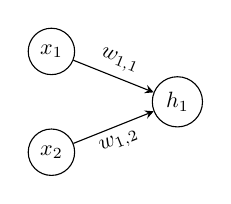
\begin{tikzpicture}[>=stealth, node distance=2cm, scale=0.8, transform shape]

            \node[draw, circle, minimum size=0.7cm] (x1) at (0,0.8) {$x_1$};
            \node[draw, circle, minimum size=0.7cm] (x2) at (0,-0.8) {$x_2$};


            \node[draw, circle, minimum size=0.7cm] (h1) at (2,0) {$h_1$};



            % Connections: inputs to hidden
            \draw[->] (x1) -- (h1) node[midway, sloped, above] {$w_{1,1}$};
            \draw[->] (x2) -- (h1) node[midway, sloped, below] {$w_{1,2}$};

        \end{tikzpicture}

        \begin{align*}
            z_1 & = w_{1,1}x_1 + w_{1,2}x_2 + b_1                                                                           \\
            z_1 & = \begin{bmatrix} w_{1,1} \quad w_{1,2} \end{bmatrix}\cdot \begin{bmatrix} x_1 \\ x_2 \end{bmatrix} + b_1 \\
        \end{align*}
    \end{center}
\end{minipage}
\begin{minipage}{0.3\textwidth}
    \begin{center}
        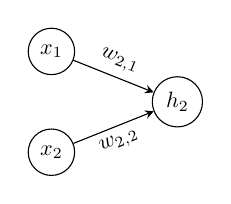
\begin{tikzpicture}[>=stealth, node distance=2cm, scale=0.8, transform shape]

            \node[draw, circle, minimum size=0.7cm] (x1) at (0,0.8) {$x_1$};
            \node[draw, circle, minimum size=0.7cm] (x2) at (0,-0.8) {$x_2$};


            \node[draw, circle, minimum size=0.7cm] (h2) at (2,0) {$h_2$};



            % Connections: inputs to hidden
            \draw[->] (x1) -- (h2) node[midway, sloped, above] {$w_{2,1}$};
            \draw[->] (x2) -- (h2) node[midway, sloped, below] {$w_{2,2}$};


        \end{tikzpicture}

        \begin{align*}
            z_2 & = w_{2,1}x_1 + w_{2,2}x_2 + b_2                                                                           \\
            z_2 & = \begin{bmatrix} w_{2,1} \quad w_{2,2} \end{bmatrix}\cdot \begin{bmatrix} x_1 \\ x_2 \end{bmatrix} + b_2 \\
        \end{align*}
    \end{center}
\end{minipage}
\begin{minipage}{0.3\textwidth}
    \begin{center}
        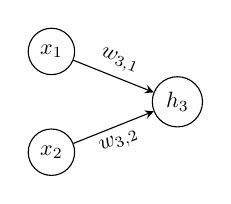
\begin{tikzpicture}[>=stealth, node distance=2cm, scale=0.8, transform shape]

            \node[draw, circle, minimum size=0.7cm] (x1) at (0,0.8) {$x_1$};
            \node[draw, circle, minimum size=0.7cm] (x2) at (0,-0.8) {$x_2$};


            \node[draw, circle, minimum size=0.7cm] (h3) at (2,0) {$h_3$};



            % Connections: inputs to hidden
            \draw[->] (x1) -- (h3) node[midway, sloped, above] {$w_{3,1}$};
            \draw[->] (x2) -- (h3) node[midway, sloped, below] {$w_{3,2}$};

        \end{tikzpicture}

        \begin{align*}
            z_3 & = w_{3,1}x_1 + w_{3,2}x_2 + b_3                                                                           \\
            z_3 & = \begin{bmatrix} w_{3,1} \quad w_{3,2} \end{bmatrix}\cdot \begin{bmatrix} x_1 \\ x_2 \end{bmatrix} + b_3 \\
        \end{align*}
    \end{center}
\end{minipage} \\
Lets let the vector $\mathbf{z}$ represent the outputs of these neuerons:
$$
    \mathbf{z} =
    \begin{bmatrix}
        z_1 \\ z_2 \\ z_3
    \end{bmatrix}
    =
    \begin{bmatrix}
        w_{1,1} & w_{1,2} \\
        w_{2,1} & w_{2,2} \\
        w_{3,1} & w_{3,2} \\
    \end{bmatrix} \cdot \begin{bmatrix}
        x_1 \\ x_2
    \end{bmatrix} +
    \begin{bmatrix}
        b_1 \\ b_2 \\ b_3
    \end{bmatrix}
$$
This is the essence of a forward pass, we've desribed a network of two input neuerons and three hidden neuerons.

\begin{figure}[h]
    \centering
    \begin{subfigure}[b]{0.35\textwidth}
        \centering
        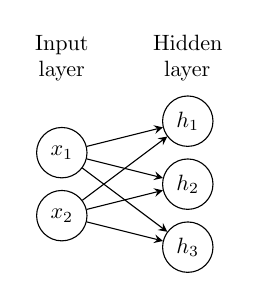
\begin{tikzpicture}[>=stealth, node distance=2cm, scale=0.8, transform shape]
            \node[align=left] at (0,2) {Input \\ \,layer};
            \node[draw, circle, minimum size=0.8cm] (x-1) at (0,0.5) {$x_1$};
            \node[draw, circle, minimum size=0.8cm] (x-2) at (0,-0.5) {$x_2$};

            \node[align=left] at (2,2) {Hidden \\ \, layer};
            \node[draw, circle, minimum size=0.8cm] (h1) at (2,1) {$h_1$};
            \node[draw, circle, minimum size=0.8cm] (h2) at (2,0) {$h_2$};
            \node[draw, circle, minimum size=0.8cm] (h3) at (2,-1) {$h_3$};



            % Connections: inputs to hidden
            \draw[->] (x-1) -- (h1);
            \draw[->] (x-1) -- (h2);
            \draw[->] (x-1) -- (h3);


            \draw[->] (x-2) -- (h1);
            \draw[->] (x-2) -- (h2);
            \draw[->] (x-2) -- (h3);




        \end{tikzpicture}

        \subcaption{Architecture of the chef analogy}
    \end{subfigure}
    \begin{subfigure}[b]{0.64\textwidth}
        \centering
        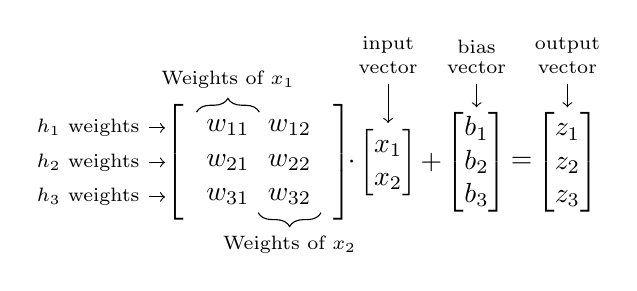
\begin{tikzpicture}[baseline=(current bounding box.center), node distance=0.1cm ]
            % Create the matrix of weight nodes with annotations
            \matrix (m) [matrix of math nodes,
            left delimiter={[}, right delimiter={]}]
                {
                    w_{11} & w_{12} \\
                    w_{21} & w_{22} \\
                    w_{31} & w_{32} \\
                };

            % Braces for the weights corresponding to x_1 and x_2
            \draw [decorate,decoration={brace,amplitude=5pt}]
            ($(m-1-1.west)+(0,0.2)$) -- ($(m-1-1.east)+(0,0.2)$)
            node[midway, above, yshift=0.5em]{\scriptsize Weights of $x_1$};

            \draw [decorate,decoration={brace,amplitude=5pt, mirror}]
            ($(m-3-2.west)+(0,-0.2)$) -- ($(m-3-2.east)+(0,-0.2)$)
            node[midway, below, yshift=-0.5em]{\scriptsize Weights of $x_2$};

            \draw [<-]
            ($(m-1-1.west)+(-0.4, 0)$) -- ($(m-1-1.west)+(-0.6, 0)$)
            node[midway, left=0.1cm] {\scriptsize $h_1$ weights};
            \draw [<-]
            ($(m-2-1.west)+(-0.4, 0)$) -- ($(m-2-1.west)+(-0.6, 0)$)
            node[midway, left=0.1cm] {\scriptsize $h_2$ weights};
            \draw [<-]
            ($(m-3-1.west)+(-0.4, 0)$) -- ($(m-3-1.west)+(-0.6, 0)$)
            node[midway, left=0.1cm] {\scriptsize $h_3$ weights};

            % Nodes for the computation on the right of the weight matrix
            \node (mult) [right= of m] {$\cdot$};
            \node (input) [right=-0.2cm of mult] {$\begin{bmatrix} x_1 \\ x_2 \end{bmatrix}$};
            \node (plus) [right=-0.2cm of input] {$+$};
            \node (bias) [right=-0.2cm of plus] {$\begin{bmatrix} b_1 \\ b_2 \\ b_3 \end{bmatrix}$};
            \node (equal) [right=-0.2cm of bias] {$=$};
            \node (zvec) [right=-0.2cm of equal] {$\begin{bmatrix} z_1 \\ z_2 \\ z_3 \end{bmatrix}$};

            \draw[<-] ($(input) + (0,0.5)$)  -- ($(input) + (0,1)$) node [above] {\shortstack{\scriptsize input \\ \scriptsize vector}};
            \draw[<-] ($(bias) + (0,0.7)$)  -- ($(bias) + (0,1)$) node [above] {\shortstack{\scriptsize bias \\ \scriptsize vector}};
            \draw[<-] ($(zvec) + (0,0.7)$)  -- ($(zvec) + (0,1)$) node [above] {\shortstack{\scriptsize output \\ \scriptsize vector}};
        \end{tikzpicture}
        \subcaption{Matrix representation of the forward pass}
    \end{subfigure}
    \caption{Representation of the forward pass}
\end{figure}


\pagebreak
\section{TO DO}
\scriptsize
\begin{itemize}
    \item Current Section
          \begin{itemize}
              \item Finish the forward pass  sub section
              \item Subsection on how  each layers output is compted $z^{(l)} = W^{(l)}a^{(l-1)} + b^{(l)}$ and $a^{(l)} = \phi(z^{(l)})$
              \item emphasis on vectorization for efficiency
              \item Subsection on cost functions and error metrics
          \end{itemize}
    \item New sub section on learning
          \begin{itemize}
              \item Summary of how we adjust weights
              \item Backprop
              \item Why we use smooth activation functions
              \item discuss sigmoid, tanh, relu, leaky relu (pros cons - sigmoid staturation, tanh zero centered, relu simple, leaky relu to prevent dying neurons)
              \item When to use each (typical guidlines - relu for hidden layers, tanh for output, leaky relu for deeper networks, softmax for multiclass classification)
              \item  derivaties of common activation functions
              \item chain rule application from output layer back to input layer
              \item how to update weights and biases using the computed gradients
              \item the role of the learning rate
          \end{itemize}
    \item Choice of cost function
          \begin{itemize}
              \item Mean Squared Error, Cross Entropy
              \item explain the difference between the two, i.e. MSE for regression, cross entropy for classification
          \end{itemize}

    \item Error Backpropogation
          \begin{itemize}
              \item how the network distributes the error back through the network
              \item deriving partial derivaties for weights and biases at each layer
          \end{itemize}
    \item Optimization and Training
          \begin{itemize}
              \item Batch Based Methods
              \item Stochastic Gradient Descent, Mini Batch Gradient Descent
              \item Explain the difference between the two, i.e. SGD for noisy data, Mini Batch for more stable convergence
              \item Improving convergence
              \item Momentum, RMSProp, Adam
              \item Explain the role of each, i.e. momentum to prevent oscillations, RMSProp to adjust learning rates, Adam as a combination of the two
              \item Explanation of the hyperparameters for each optimization method
          \end{itemize}
    \item Regularization
          \begin{itemize}
              \item Overfitting and Underfitting
              \item Techniques to prevent overfitting, i.e. dropout, L1/L2 regularization, early stopping
          \end{itemize}
    \item Initalization
          \begin{itemize}
              \item Why naive (all zeros) initialization fails
              \item Recommended schemes for initialization, i.e. Xavier, He
          \end{itemize}
    \item Building the Multilayer Perceptron for MNIST
          \begin{itemize}
              \item Data input: Organize your data and labels
              \item Network structure: define layers, number of
              \item Forward Propogation: Implement the sequence of matrix multiplications, biases and activations
              \item Loss calculation: e.g. cross entropy for classification tasks
              \item Backpropogation: Compute gradients layer by layer
              \item Weight updates: Incorporate an optimization method (SGD, Adam, etc)
              \item Training loop: Shufflee data, iterate over epochs, track training and validation loss
          \end{itemize}
    \item Extensions and Next steps
          \begin{itemize}
              \item Deeper architectures: convoulition nueral networks, recurrent neural networks, transformers
              \item Modern practices: Batch normalization, advanced regularization, learning rate schedules
          \end{itemize}
    \item Modern Practices
          \begin{itemize}
              \item Batch Normalization
              \item Advanced Regularization
              \item Learning Rate Schedules
          \end{itemize}
\end{itemize}


\pagebreak

\bibliographystyle{plain} % Choose a style (plain, IEEEtran, etc.)
\bibliography{references} % Ensure this matches your .bib file name

\end{document}



